\chapter{Αξιολόγηση επιδόσεων}

\section{Σύγκριση με υπάρχουσες \en{unikernel} λύσεις}

Για την αξιολόγηση του μηχανισμού \en{utmem} ως \en{unikernel}
χρησιμοποιούμε ως καταλληλότερο το μετροπρόγραμμα (\en{benchmark)}
\en{Redis (Remote Dictionary Server)}.
Το \en{Redis} είναι ιδανικό για αυτόν το σκοπο για δύο
λόγους. Πρώτον πρόκειται, όπως λέει και ίδιο \cite{redis}, για ένα
\en{data structure store}, δηλαδή ένα εξυπηρετητή αποθήκευσης αφηρημένων
δεδομένων, όπου οι βασικές λειτουργίες είναι \en{get} και \en{set}
με αναφορά σε κλειδιά, και άρα υπάρχει προφανής ομοιότητα
με τα \en{utmem operations}. Δεύτερον, υπάρχει ήδη έκδοση \en{unikernel}
του \en{Redis} από τα προσφερόμενα \en{Rumprun-packages} στο επίσημο \en{repository},
οπότε δεν χρειάζεται να το μετατρέψουμε εμείς σε \en{unikernel}\cite{redisUni}.
\newline

Η γενική δομή του \en{Redis} μοντέλου, είναι η ύπαρξη ενός \en{back-end server},
ο οποίος είναι υπεύθυνος για την αποθήκευση αφηρημένης
μορφής δεδομένων, και την εξυπηρέτηση αιτημάτων από τρίτες
εφαρμογές επάνω σε αυτά τα δεδομένα. Ταυτόχρονα, υπάρχουν
διάφοροι \en{front-end clients}, οι οποίοι αποστέλνουν αιτήματα
στον server με το \en{TCP/IP} πρωτόκολλο. Ως \en{unikernel}
προσφέρεται μόνο ο \en{Redis server}, και ο \en{client} μπορεί να
είναι οποιαδήποτε εφαρμογή ικανή να διαχειρίζεται \en{TCP} αιτήματα, π.χ. \en{nc}.
\newline

Αποφασίζουμε να προσθέσουμε τρεις νέες εντολές στο\en{ Redis},
τις \en{tmemPut, tmemGet, tmemInval},
οι οποίες όπως δείχνει το ονομά τους αντιστοιχούν
στα τρια \en{utmem operation} που υλοποιήσαμε. Στα εξής θα
αναφερόμαστε σε αυτές τις εντολές ως \en{tmem commands},
για να τις ξεχωρίζουμε από τα \en{tmem operations}. Ο προτεινόμενος
τρόπος εισαγωγής εντολών στο \en{Redis} είναι η δημιουργία
ενός \en{Redis module} το οποίο προσθέτει τις εντολές κατά
το \en{runtime} του \en{Redis server}. Όμως η έκδοση του \en{Redis},
που υπάρχει ως \en{unikernel}, είναι αρκετά παλιά και δεν
υποστηρίζει τα \en{modules}, οπότε προσθέσαμε τις εντολές απευθείας
στον πηγαίο κώδικα του \en{Redis server}.
\newline

Επίσης επιλέγουμε να χρησιμοποιηθεί η έκδοση \en{utmem} μέσω
\en{function call}, και όχι \en{system call}. Αυτό εξαλείφει
την πιθανότητα τα αποτελέσματά μας να επηρεάζονται από
τις αλλαγές στα \en{rump kernels}, μιας και τα χρησιμοποιούμε
χωρίς αλλαγή. Πρέπει μόνο να ενσωματώσουμε την
μεταγλώττιση του\en{ driver} της \en{utmem} στο \en{Redis}, το οποίο
σημαίνει να προστεθούν \en{flags} για \en{assembly compilation}.
\newline

Οι μετρήσεις έγιναν μέσα σε εικονική μηχανή \en{QEMU/KVM}
με \en{Ubuntu Linux 4.9.39}, στον πυρήνα του οποίου
έχουν προστεθεί τα \en{patch} της αυθεντικής \en{utmem} για το
\en{back-end}. Ο επεξεργαστής είναι \en{intel core i5-8250u} από τον οποίο
αναθέτουμε 2 φυσικούς πυρήνες (4 λογικούς), ενώ η
διαθέσιμη μνήμη \en{RAM} του \en{VM} είναι \en{4GB}.
\newline

Τέλος, οφείλουμε να διευκρινίσουμε πως εκτελουμε το
\en{Redis} χωρίς \en{AOF persistence}. Το \en{Redis} προσφέρει
δυνατότητα διατήρησης των δεδομένων της μνήμης τους
στο δίσκο ώστε αυτά να μπορούν να ανακτηθούν σε περίπτωση
μη προβλεπόμενου τερματισμού του \en{Redis}. Διατηρεί,
συνεπώς ένα αρχείο με αυτές τις εγγραφές στον δίσκο.
Το μειονέκτημα, όπως είναι πως κάθε προσθετοαφαίρεση
δεδομένου, π.χ. μια \en{set}, μπλοκάρει μέχρι να γραφούν τα
δεδομένα στο δίσκο\cite{redisAOF}. Ως γνωστόν, οι δίσκοι είναι τάξης
μεγέθους πιο αργοί από την κύρια μνήμη, συνεπώς το να
διατηρούσαμε το \en{AOF persistance} του \en{Redis} θα έδινε ένα
άδικο πλεονέκτημα στα \en{tmem commands} μας, τα οποία δεν
διατηρούν τέτοια αντίγραφα. Συγκρίνουμε, λοιπόν μόνο
\en{in-memory} ενέργειες του \en{Redis}.



\subsection{Σενάριο 1: με άφθονη μνήμη}

Για μετρήσουμε την συμπεριφορά του \en{Redis} με τα νέα \en{commands},
δημιουργήσαμε ένα \en{custom} μετροπρόγραμμα, το οποίο ονομάζουμε
\en{client}. Το πρόγραμμα αποστέλνει μέσω \en{TCP/IP network requests},
προς το \en{Redis}. Ταυτόχρονα, ο client καταγράφει δεδομένα για την επίδοση
της επικοινωνίας με τον \en{server}. O \en{client} τρέχει στον \en{host} ως απλή διεργασία
ώστε να μην επηρεάζεται η εκτέλεση του \en{Redis}, το οποίο
με την σειρά του τρέχει ως \en{unikernel}. Θέλουμε να συγκρίνουμε
δύο \en{commands}, το απλό \en{set} και το \en{tmemPut}, οπότε για δίαφορους
συνδυασμούς μεγέθους \en{value} και αριθμό \en{requests} λαμβάνουμε
μετρήσεις για το πόσο χρόνο χρειάστηκε να ικανοποιηθούν όλα
τα \en{requests}, και στην συνέχεια παίρνουμε ένα μέσο όρο.
Συνεπώς, η μετρική που μας ενδιαφέρει είναι τα \en{commands}/δευτερόλεπτο.
\newline

Αναλυτικότερα, επιλέγουμε ένα μέγεθος τιμής (\en{value size}) και ένα αριθμό από
τιμές (\en{number of values}) που θα καταχωρήσουμε στο \en{Redis}.
Για παράδειγμα ο συνδυασμός 512-1024 σημαίνει πως θα
καταχωρηθούν 1024 τιμές, η κάθε μια από τις οποίες αντιστοιχεί σε ένα ξεχωριστό command,
όπου κάθε τιμή θα έχει μέγεθος 512 bytes. Αυτή η διαδικασία γίνεται για πολλούς συνδυασμούς
\en{value size} και \en{number of values}. Προφανώς, ανάμεσα σε κάθε επανάληψη του πειράματος φροντίζουμε
να αδειάζει η μνήμη του \en{Redis} ή το \en{tmem pool}, για
το \en{set} ή το \en{tmemPut} αντίστοιχα.
\newline

Η δομή του συστήματος \en{client} και \en{Redis unikernel} φαίνεται στην εικόνα
\ref{fig:benchSetup}.
\newline

\begin{figure}[h]
  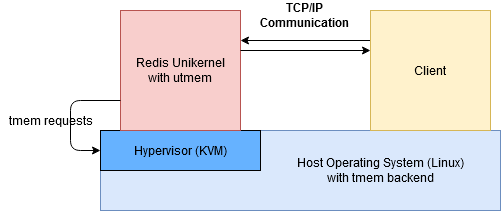
\includegraphics[width=\textwidth]{pictures/benchmarkSetup.png}
  \caption{Επικοινωνία και δομή \en{client - Redis unikernel}}
  \label{fig:benchSetup}
\end{figure}

Εν τέλει παρατηρείται πως, όταν υπάρχει αρκετή μνήμη τα \en{tmem commands} είναι σχετικά
πιο αργά από τις \en{set} εντολές του \en{Redis}. Αυτό είναι λογικό,
καθώς πρώτον πρέπει για κάθε \en{tmem command} να
εκτελείται ένα \en{hypercall}, το οποίο είναι σύγχρονος μηχανισμός
και άρα οδηγεί σε μπλοκάρισμα του \en{unikernel}. Δεύτερον, πρέπει
να αντιγράφεται το σύνολο των δεδομένων από τον χώρο του
\en{unikernel} στον χώρο πυρήνα του \en{host}, αυξάνοντας τις αντιγραφές που
εκτελούνται ανά \en{command}. Στην εικόνα \ref{fig:tmemPut-Set} φαίνεται
η σχετική συμπεριφορά των δύο ειδών \en{commands} για διάφορους συνδυασμούς μεγέθους \en{value}
και αριθμού \en{requests}, ενώ στην εικόνα \ref{fig:tmemPut-SetPercentage} παρουσιάζεται η ποσοστιαία
διαφορά ταχύτητας των δύο εντολών παίρνοντας μέσο όρο ανά \en{value size}.
\newline

\begin{figure}[h]
  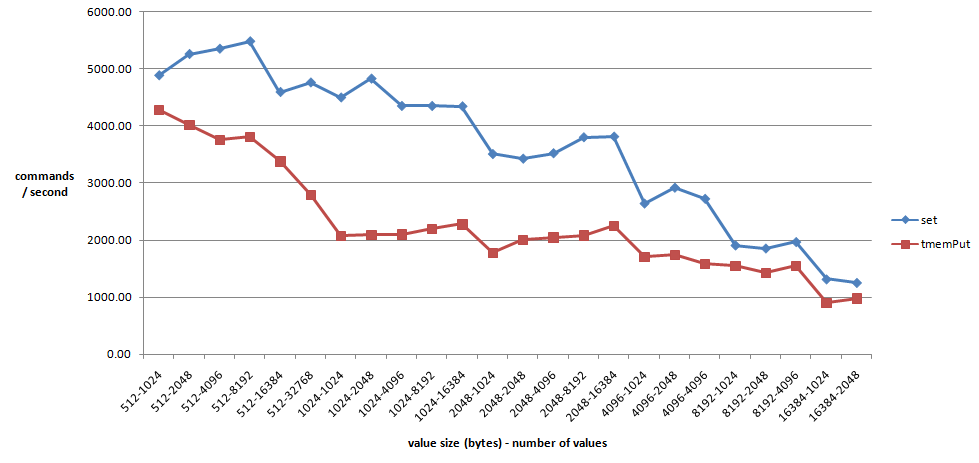
\includegraphics[width=\textwidth]{pictures/firstBenchmarkResults.PNG}
  \caption{Σύγκριση \en{tmemPut} και \en{set commands}. Φαίνεται πως
  η \en{tmemPut} σχετικά πιο αργή από την \en{set} μετρώντας
  \en{commands/second}}
  \label{fig:tmemPut-Set}
\end{figure}

\begin{figure}[h]
  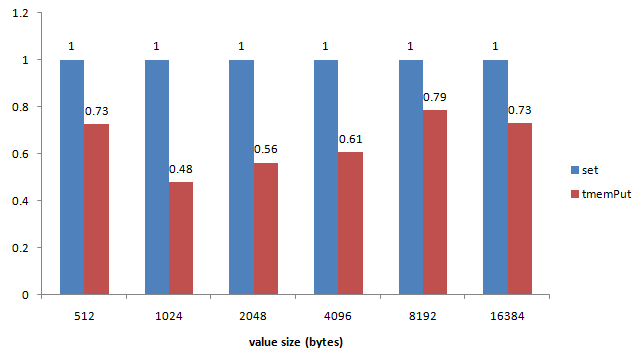
\includegraphics[width=\textwidth]{pictures/firstBenchmarkResults2.PNG}
  \caption{Ποσοστιαία σχέση \en{tmemPut} και \en{set} κανονικοποιημένη ως προς \en{set}}
  \label{fig:tmemPut-SetPercentage}
\end{figure}


\subsection{Σενάριο 2: με έλλειψη μνήμης}

Επιθυμούμε να μελετήσουμε την συμπεριφορά του \en{Redis} και σε περιπτώσεις
όπου ο πόρος της μνήμης είναι σημαντικά περιορισμένος. Τρέχουμε πάλι τον ίδιο
\en{Unikerel server}, αλλά τώρα περιορίζουμε την διαθέσιμη μνήμη όλης της εικονικής
μηχανής σε μερικές δεκάδες \en{mega bytes}.
\newline

Όταν η μνήμη είναι περιορισμένη, τα \en{tmem commands} γίνονται η
μόνη λειτουργική λύση για αποθήκευση δεδομένων. Θυμίζουμε
πως στο \en{Rumprun} απουσιάζει η εικονική μνήμη, συνεπώς όταν
γεμίσει η διαθέσιμη δεν υπάρχει κάποιος μηχανισμός να απελευθερώσει
αυτήν την πίεση μνήμης. Στην περίπτωση του \en{set}, μετά από ένα
αριθμό από \en{requests}, είναι αδύνατον να κατανεμηθεί νέα μνήμη, έστω
εικονική, στο \en{Redis}, το οποίο πλέον αδυνατεί να ικανοποιήσει
τα \en{requests} που του έρχονται από τον \en{client}. Σε αυτό το σενάριο, εμφανίζει
μήνυμα σφάλματος και τερματίζει την λειτουργία του. Καταστροφική
συμπεριφορά για ένα εξωτερικό χρήστη που επικοινωνεί με το
\en{unikernel}. Αντίθετα, το \en{tmemPut} ικανοποιείται κανονικά, καθώς η
απαίητηση σε χώρο είναι ελάχιστη, αρκεί δηλαδή να ικανοποιείται
ένα \en{request}, για να ικανοποιηθούν όλα, μιας και τα δεδομένα
αποθηκεύονται στην μνήμη του \en{host}. Μάλιστα η συμπεριφορά είναι
ταυτόσημη με την περίπτωση αφθονίας μνήμης, δεν παρατηρείται κάμια επιπλέον
καθυστέρηση λόγω της περιορισμένης μνήμης.







\section{Σύγκριση με την αυθεντική \en{utmem}}

Για να εξαχθεί μια πλήρης εικόνα των επιδόσεων του μηχανισμού, θεωρούμε σκόπιμο,
να συγκρίνουμε την \en{utmem} υλοποίηση σε \en{unikernel}, σε σχέση με τον
αυθεντικό (\en{original}) μηχανισμό της \en{utmem}.
\newline

Χρησιμοποιούμε πάλι το μετροπρόγραμμα \en{Redis}, για το οποίο υπάρχει
\en{Redis-module} με το οποίο το \en{Redis} τίθεται ικανό να ικανοποιήσει \en{utmem}
αιτήματα χρησιμοποιώντας τον αυθεντικό μηχανισμό. Αναφερόμαστε πλέον στο
\en{Redis} ως κανονική διεργασία ενός \en{linux} συστήματος. Θυμίζουμε, πως ο
αυθεντικός μηχανισμός χρησιμοποιεί μια εικονική συσκευή (\en{/dev/utmem}) του \en{linux},
ούτως ώστε οι διεργασίες να μπορούν να ζητάν από τον πυρήνα να
εκτελέσει \en{tmem} αιτήματα προς το \en{backend} εκ μέρους αυτών. Επιπροσθέτως,
επιθυμούμε ο τρόπος μέτρησεις να είναι όσο το δυνατόν όμοιως με τον τρόπο
μέτρησης που περιγράφεται στην εργασία της αυθεντικής \en{utmem} \cite{Aimilios}, συνεπώς
δημιουργήσαμε ένα διαφορετίκό πρόγραμμα \en{client} που αποστέλει αιτήματα. Αυτή τη φορά,
δεν γεμίζουμε την \en{tmem pool} με δεδομένα, αλλά αποστέλλουμε συνεχώς το ίδιο αίτημα,
δηλαδή το ίδιο \en{key}, για προκαθορισμένο χρονικό διάστημα και εν τέλει υπολογίζουμε ένα
μέσο όρο αιτημάτων. Αποστέλουμε ακριβώς τα ίδια αιτήματα και στο \en{unikernel Redis}, ωστέ
να μπορούμε να έχουμε μια όμοια σύγκριση μεταξύ των δύο εκδόσεων. Ελέγχουμε διάφορες τιμές του μεγέθους της τιμής (\en{value size}),
ενώ το \en{utmem command} είναι τύπου \en{Put}. Όπως και προηγουμένως, η μετρική που
μας ενδιαφέρει είναι τα \en{commands / second} που εξυπηρετούνται.
\newline

Η τοπολογία του συστήματος μετρήσεων είναι η εξής:
όταν μετράμε την αυθεντική \en{utmem}, το \en{Redis} εκτελείται ως μια
κανονική διεργασία εντός εικονικής μηχανής (\en{guest}) με 2 \en{GB RAM} και ίδιου
πυρήνα με τον \en{host}, δηλαδή τον πυρήνα με τα \en{utmem patches}. Για την \en{utmem}
ως \en{unikernel}, εκτελούμε ένα \en{unikernel} επάνω στον ίδιο \en{host}.
Τέλος, ο \en{client} εκτελείται επίσης ως απλή διεργασία
επάνω στον \en{Ηost}. Η διάταξη φαίνεται καλύτερα στο σχήμα \ref{fig:original-unikernelTopo}.
\newline

\begin{figure}[h]
  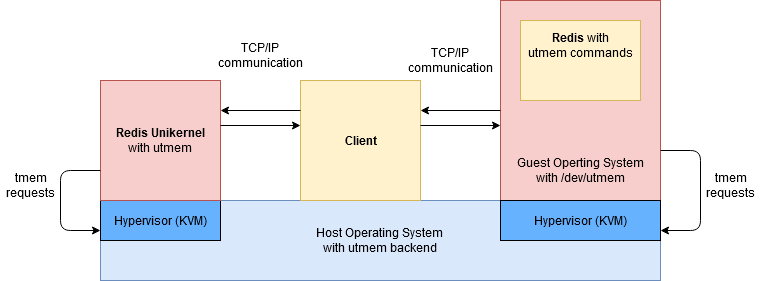
\includegraphics[width=\textwidth]{pictures/bench2Setup.PNG}
  \caption{Τοπολογία σύγκρισης αυθεντικής \en{utmem} και \en{Unikernel utmem}}
  \label{fig:original-unikernelTopo}
\end{figure}

Στο σχήμα \ref{fig:original-unikernel} φαίνονται τα αποτελέσματα των μετρήσεων. Παρατηρούμε
πως η έκδοση \en{utmem} για \en{unikernel} είναι σταθερά ταχύτερη από τον αυθεντικό
μηχανισμό. Μάλιστα, όσο το
μέγεθος του \en{value} μεγαλώνει τόσο η μεγαλώνει και η διαφορά στην επίδοση
ανάμεσα στους δύο μηχανισμούς.
Στο σχήμα \ref{fig:original-unikernelPercentage}
φαίνεται και η ποσοστιαία διαφορά των δύο εκδόσεων ανά \en{value size}.
\newline

\begin{figure}[h]
  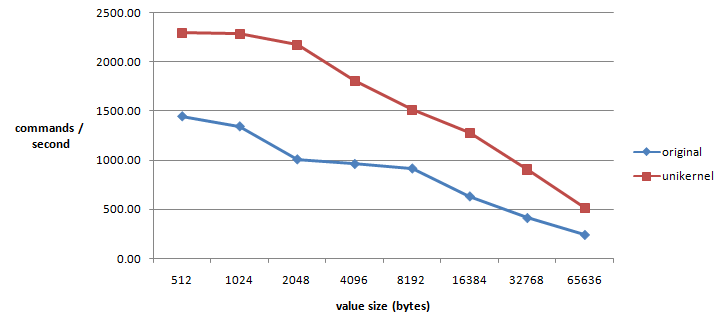
\includegraphics[width=\textwidth]{pictures/secondBenchmarkResults.PNG}
  \caption{Επίδοση αυθεντικής \en{utmem} και \en{Unikernel utmem}}
  \label{fig:original-unikernel}
\end{figure}

\begin{figure}[h]
  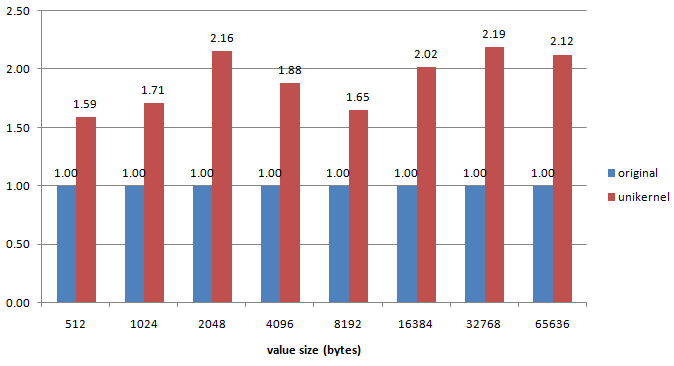
\includegraphics[width=\textwidth]{pictures/secondBenchmarkResults2.PNG}
  \caption{Ποσοστιαία σχέση αυθεντικής \en{utmem} και \en{unikernel utmem} κανονικοποιημένη ως προς
  την αυθεντική}
  \label{fig:original-unikernelPercentage}
\end{figure}

Υπάρχει μια εγγενής ασυμμετρία στα δυο συστήματα που μελετάμε καθώς πρόκειται
για δύο διαφορετικής σχεδίασης και πολυπλοκότητας εικονικές μηχανές. Η εικονική μηχανή μέσα
στην οποία εκτελείται η αυθεντική \en{utmem} διαθέτει διαφορετικό υποσύστημα δικτύου, ενώ εκτελεί παράλληλα
και άλλες διεργασίες εντός της. Ταυτόχρονα, το πλεονέκτημα της \en{unikernel} έκδοσης,
είναι πως χρειάζονται λιγότερες αντιγραφές του \en{value} από το επίπεδο του
\en{Redis} μέχρι και το \en{backend}, το οποίο είναι κοινό και για τις δύο εκδόσεις, ενώ παράλληλα απουσιάζει και η
ανάγκη για \en{context switch}. Αυτή η σχεδιαστική διαφορά εξηγεί την αύξηση της απόδοσης όσο μεγαλώνει το \en{value size}.
Το \en{unikernel} περιβάλλον, προσφέρει ένα σαφές πλεονέκτημα στην ταχύτητα εξυπηρέτησης
των αιτημάτων, το οποίο δείχνει πως αυτές οι δύο τεχνολογίες συνεργάζονται αρμονικότατα.
\newline

Για να εξακριβώσουμε την επιτάχυνση που προσφέρει το \en{Rumprun framework} σε σχέση με
ένα παραδοσιακό \en{VM} συγκρίναμε την εντολή \en{set} του \en{Redis}, τόσο σε \en{unikernel}
περιβάλλον όσο και σε παραδοσιακό \en{VM}, όπως και πριν δηλαδή.
Θεωρούμε πως δίνει μια καλή ποιοτική ένδειξη, καθώς η διαδικασία εξυπηρέτησης της συγκεκριμένης εντολής είναι η ίδια
και στις δύο περιπτώσεις. Το αποτέλεσμα φαίνεται στην εικόνα \ref{fig:original-unikernelSet}. Η συμπεριφορά ταιριάζει με την συμπεριφορά που παρατηρείται
για τα \en{utmem commands}, όπως και αναμένονταν. Φαίνεται πως κατά μέσο όρο, για την περιοχή μεγεθών
που μελετάμε το \en{Rumprun} εμφανίζει περίπου διπλάσιες επίδοσεις σε σχέση με τα συμβατικό \en{VM}.


\begin{figure}[h]
  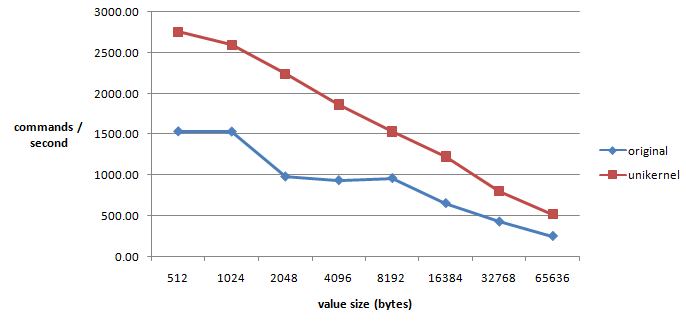
\includegraphics[width=\textwidth]{pictures/secondBenchmarkResults3.PNG}
  \caption{Επίδοση \en{set} εντολής, μεταξύ \en{unikernel} και συμβατικού περιβάλλοντος}
  \label{fig:original-unikernelSet}
\end{figure}




\section{Σχολιασμός}

Από το παραπάνω προκύπτει το εξής ενδιαφέρον συμπέρασμα. Με
χρήση της \en{utmem}, και του \en{Rumprun unikernel framework}, είναι
δυνατόν να εκτελούνται σε εικονοποιημένο περιβάλλον \en{unikernels},
στα οποία αρχικά δίνεται ελάχιστη μνήμη. Στην περίπτωση
του \en{Redis} αρκούν μόνο 64 \en{mega bytes}. Ο φαινομενικός αυτός περιορισμός,
δεν απαγορεύει να εκτελούνται \en{memory intensive} διεργασίας
ως \en{unikernel}, καθώς τα \en{tmem pools} αποθηκεύουν τα δεδομένα που
κανονικά θα βρίσκονταν στην μνήμη εκτός αυτής. Ουσιαστικά εξασφαλίζεται
αδιάκοπη εκτέλεση των \en{unikernels}, και αποφεύγεται η σπατάλη
μνήμης που εν τέλει δεν χρησιμοποιείται από το \en{unikernel}.
Παράλληλα, μεγιστοποιείται ο αριθμός των \en{unikernel}, και
γενικά των εικονικών μηχανών, που μπορούν να εκτελούνται
παράλληλα σε ένα φυσικό σύστημα ανά μονάδα μνήμης.
\newline

Αυτό που πέτυχε στη αυθεντική εργασία η \en{utmem}\cite{Aimilios}, ήταν να
δώσει στον προγραμματιστή ένα χρησιμότατο εργαλείο.
Προσαρμόζοντας ελαφρώς την συμπεριφορά της εφαρμογής
τους ως προς την διαχείριση της μνήμης κέρδισε σε επιδόσεις
και ταχύτητα, σε σχέση με το να εμπιστεύονταν αποκλειστικά
τα υποσυστήματα διαχείρισης μνήμης (\en{frontswap}). Τώρα,
αυτό το εργαλείο προσφέρεται και στο \en{Rumprun unikernel framework},
στο οποίο το σενάριο έλλειψης μνήμης οδηγεί σε καταστροφικές συμπεριφορές.
\newline

Σημαντικό, επίσης, είναι το γεγονός πως η έκδοση \en{utmem} ως \en{unikernel} έχει
επιδόσεις ανώτερες από τον αυθεντικό μηχανισμό. Η επιτάχυνση που προσφέρει το \en{Rumprun} κρίνεται
ζωτικής σημασίας για εφαρμογές ευαίσθητες στον χρόνο απόδοσης, όπως δείξαμε για μια αποθήκη δεδομένων
όπως το \en{Redis}. Τα οφέλη, συνεπώς, πολλαπλασιάζονται, όχι μόνο ελαχιστοποιούνται οι ανάγκες μας σε μνήμη, αλλά
η απόκριση των εικονικών μηχανών, σε σχέση με αντίστοιχους μηχανισμούς, μεταβάλλεται θετικά.
Συμπεραίνουμε πως ο συνδυασμός \en{utmem} και \en{Rumprun} είναι κάθε άλλο από ασύμφορος ή άκαρπος.
